\documentclass[a4paper]{article}

\usepackage[francais]{babel}
\usepackage[utf8]{inputenc}
\usepackage{amsmath}
\usepackage{amssymb}
\usepackage[pdftex]{graphicx}
\usepackage{url}
\usepackage{subfigure}

% shorten margin
\usepackage[]{fullpage}

\title{FUGU : Find Your Guest Unisonously\\Site de covoiturage}
\author{Mathieu BIVERT, Sophie VALENTIN}

\makeatletter
\def\thickhrulefill{\leavevmode \leaders \hrule height 1pt\hfill \kern \z@}
\def\maketitle{%
  \null
  \thispagestyle{empty}%
  \vskip 1cm
  \begin{center}
        \normalfont\large\huge\@author
  \end{center}
  \vfil
  \vfil
  \vfil
  \vfil
  \vfil
  \vfil
  \vfil
  \vfil
  \vfil
  \vfil
  \vfil
  \vfil  
  \vfil  
  \hrule height 2pt
  \par
  \begin{center}
        \huge \strut Projet WASP\\
        \@title \par
  \end{center}
  \hrule height 2pt
  \par
  \vfil
  \vfil
  \vfil
  \vfil
  \vfil
  \vfil
  \vfil
  \vfil  
  \vfil
  \vfil
  \vfil
  \vfil  
  \vfil  
  \vfil
  \vfil  
  \vfil  
  \vfil
  \vfil
  \vfil
  \vfil
  \vfil
  \vfil
  \begin{center}
  			\huge Professeur : Tamara REZK
  \end{center}
  \null
\cleardoublepage
}
\makeatother

\begin{document}
\maketitle

\newpage

\section{Fonctionnalités de l'application web}

L'utilisateur souhaitant faire du covoiturage doit tout d'abord s'authentifier.
En effet, les utilisateurs possèdent leurs propres données.
L'utilisateur s'authentifie via un formulaire de connexion, illustré dans la figure 1.
Il doit renseigner son login et son mot de passe. S'il n'en possède pas,
il peut s'enregistrer sur la page d'inscription. Pour cela, il doit cliquer 
sur le lien "register".

\begin{figure}[!ht]
	\centering
	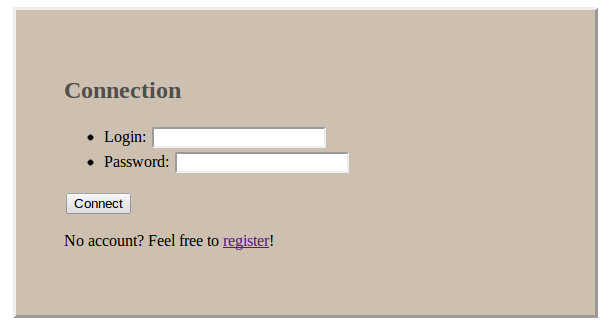
\includegraphics[scale=0.4]{Connexion.png}
	\caption{\label{login} Formulaire de connexion}
\end{figure}

\subsection{Tableau de bord de gestion}

Une fois authentifié, l'utilisateur accède à son tableau de bord, représenté en figure 2. Cet écran répertorie tous ses trajets, c'est-à-dire :
\begin{itemize}
	\item les trajets dont il est le conducteur dans la partie haute de la page;
	\item les trajets dont il est le passager dans la partie basse de la page.
\end{itemize}

\begin{figure}[!ht]
	\centering
	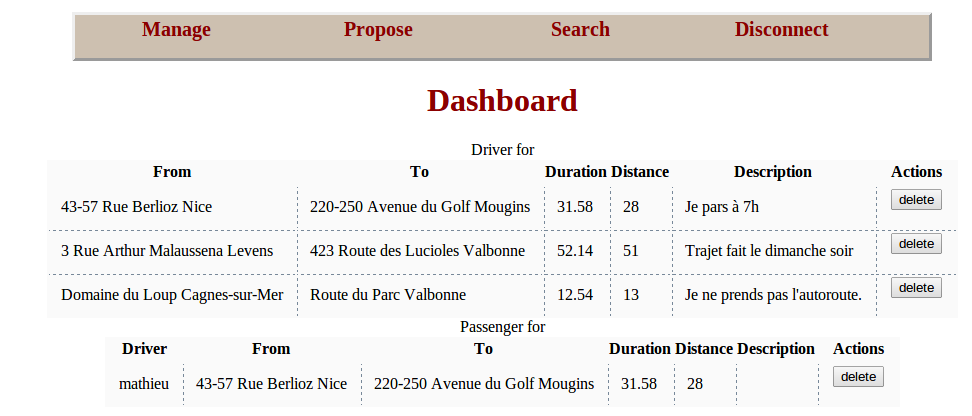
\includegraphics[scale=0.5]{Dashboard.png}
	\caption{\label{dashboard} Tableau de bord}
\end{figure}

L'utilisateur a accès à tout moment à ce tableau de bord en cliquant sur "Manage" sur le menu de navigation. Et il peut se déconnecter en cliquant sur "Disconnect".

\begin{figure}[!ht]
	\centering
	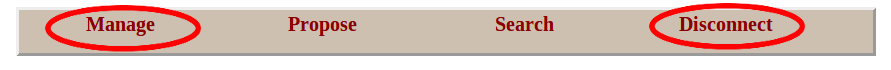
\includegraphics[scale=0.4]{Menu.png}
	\caption{\label{menu} Menu de navigation}
\end{figure}

Pour chaque trajet, les adresses de départ et d'arrivée sont affichées. Le temps (en minutes) et la distance (en kilomètres), qui ont été calculés, sont également affichés. L'utilisateur peut voir la description qui a été donnée au trajet. Généralement, ce sont des informations pratiques sur le rendez-vous.

L'utilisateur peut supprimer un trajet de son tableau de bord : pour cela, il clique sur le bouton "delete" du trajet qu'il souhaite supprimer.
Son tableau de bord est alors mis à jour. S'il était conducteur pour ce trajet, alors le trajet n'apparaîtra plus dans le tableau de bord des autres passagers. 

\subsection{Proposition de trajet}

En cliquant sur "Propose" sur le menu de navigation, l'utilisateur peut proposer un trajet comme dans la figure 4. Au chargement, une carte apparaît avec une adresse
de départ et une adresse d'arrivée par défaut. Pour indiquer son trajet, l'utilisateur a deux solutions :
\begin{itemize}
	\item il peut entrer les adresses de départ et destination dans les champs
	\item il peut déplacer les marqueurs sur la carte
\end{itemize}

Dans le premier cas, les marqueurs sur la carte sont immédiatement mis à jour. Dans le second cas, les champs d'adresses sont immédiatement mis à jour.
Et quelque soit la méthode pour indiquer le trajet, le temps de trajet et la distance sont calculés.
L'utilisateur a ensuite la possibilité de laisser une description en remplissant le champ de texte.
Pour terminer, il enregistre son trajet en cliquant sur le bouton "Propose", en-dessous de la description.

\begin{figure}[!ht]
	\centering
	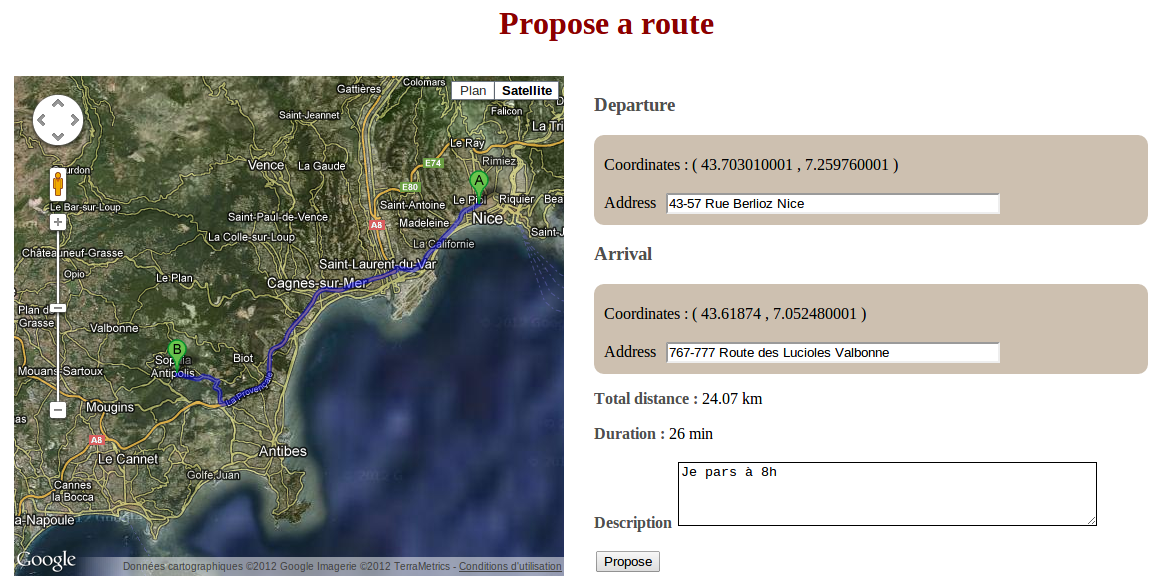
\includegraphics[scale=0.4]{Propose.png}
	\caption{\label{propose} Proposition de trajet}
\end{figure}

Après enregistrement, l'utilisateur est redirigé sur le tableau de bord où figure le nouveau trajet créé.

\subsection{Recherche de trajet}

En cliquant sur "Search" sur le menu de navigation, l'utilisateur peut chercher un trajet existant. Le principe est le même que pour la création
de trajet à l'exception que l'utilisateur ne renseigne aucun champ de description. Après un clic sur le bouton "Search", une liste de trajets
est affichée. 

\begin{figure}[!ht]
	\centering
	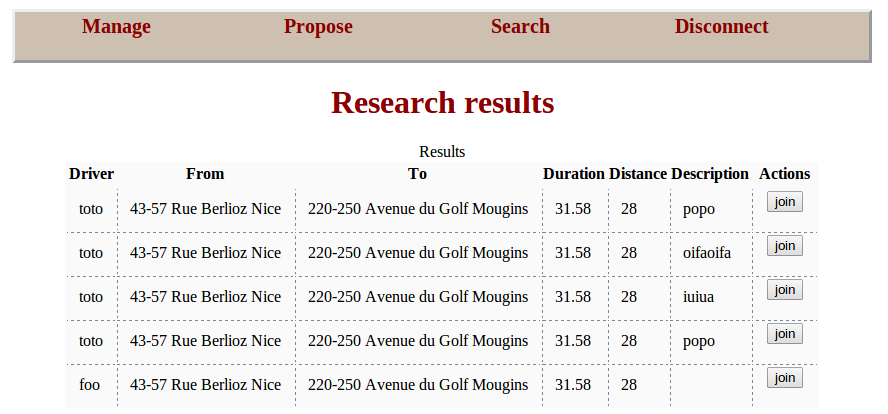
\includegraphics[scale=0.5]{Search.png}
	\caption{\label{search} Recherche de trajet}
\end{figure}

Pour chaque trajet, on peut s'inscrire en tant que passager. Il faut noter que les trajets sur lesquels on s'est déjà inscrit ne figurent
pas dans la recherche. Pour s'inscrire, on clique sur le bouton "join" en face du trajet. On est alors redirigé vers le tableau de bord
où apparaît maintenant le trajet que l'on a rejoint.

\section{Serveur}

	\subsection{Services}
	\subsection{Securité}
 		\subsubsection{Prévention de l'attaque XSRF}
 		
 		\subsubsection{Prévention des attaques contre l'intégrité de la session}
 		
On souhaite éviter que l'utilisateur ou un attaquant puisse éditer les cookies de session.
Ainsi, on stocke côté serveur une empreinte HMAC des données sensibles envoyées à l'utilisateur.
Cette empreinte est calculée grâce à deux entrées :
\begin{itemize}
	\item la donnée que l'on souhaite passer à l'utilisateur ;
	\item la clé privée connue seulement du serveur.
\end{itemize}
Lors de l'envoi d'un cookie modifié par le client ou un attaquant, le serveur détectera que l'empreinte
de la donnée envoyée par le client n'est pas la même que celle stockée côté serveur.
Ainsi on prévient les attaques visant à altérer les données de session.

		\subsubsection{Prévention des attaques de fixation}
		
Pour une telle attaque, l'attaquant fixe le Session ID dans l'URL pour un autre utilisateur.
Il envoie ensuite cette URL à l'utilisateur. Ce dernier s'authentifie et l'attaquant peut alors
utiliser la session de l'utilisateur car il connait le SID.
Pour prévenir cette attaque, il faut modifier le fichier php.ini :
\begin{itemize}
	\item en activant l'option session.use\_only\_cookies afin que le SID soit transmis exclusivement par cookie ;
	\item en s'assurant que l'option session.use\_trans\_sid est désactivée.
\end{itemize}
	
		\subsubsection{Prévention des attaques contre la confidentialité des données de session}
		
Afin qu'une attaque du type Man in the Middle n'opère pas, on utilise un flux chiffré tel que HTTPS.

		\subsubsection{Prévention des "Replay Attacks"}

		Replay attack Wiki
		Possible même avec HTTPS...
 		
 		\subsubsection{Prévention des attaques XSS}
 		
 		
 		
		\subsubsection{Prévention des attaques d'injection de code}
		\subsubsection{Prévention des attaques RFI / LFI}
		
		\subsubsection{D'autres éléments de prévention}
		
Pour limiter les vols de cookies, lors d'une déconnexion, les cookies sont effacés de la machine ciente.
Cela permet, par exemple, de limiter des vols causés par une intrusion sur le disque dur de utilisateur.
 		
\section{Client}

	\subsection{Google Maps}
	\subsection{Javascript} 
		\subsubsection{Utilisation de la Prototype Chain}
		\subsubsection{Utilisation de la Scope Chain}
		\subsubsection{Utilisation du mot-clé this}
		\subsubsection{Utilisation de la récursion}
		\subsubsection{Manipulation du DOM}
   \subsection{Securité} 
  		\subsubsection{Prévention des failles Javascript}

\end{document}
